\documentclass[14pt]{extarticle}
\usepackage{amsmath}
\usepackage{graphicx}
%\graphicspath{{./images/}}
\usepackage[left=2.5cm, right=2.5cm, top=3cm]{geometry}
\begin{document}
\section*{\centerline{Acceptance Certificate}} 

\vspace{4em}


This is to certify that the final copy of dissertation entitled "An old method of Jacobi and Lagrangian formulation of the classical cosmological equations" has been vetted by under signed and is found free of plagiarism, errors and mistakes and is accepted as partial fulfillment for award of Bachelor of Science with honours degree.\\ \\ \\


Signature of Supervisor: \\ \\
                                      
Name of Supervisor: \\ \\
                                      
Date:


\pagebreak
\section*{\centerline{Declaration}}

\vspace{3em}
\begin{itemize}
\item I hereby acknowledge and declare that the present dissertation work entitled "An old method of Jacobi and Lagrangian formulation of the classical cosmological equations" is submitted as the partial fulfillment for the degree of Bachelor of Science with honours in Physics.\\
\item I declare that this written submission represents my ideas in my own words and where other's ideas or words have been included, I have adequately cited and referenced the original sources. I declare that i have properly and accurately acknowledged all sources used in the production of this report.\\
\item I also declare that i have adhered to all principles of academic honesty and integrity and have not misrepresented or fabricated or falsified any idea/fact/source in my report. I understand that any voilation of the above will be cause for disciplinary action by the institute and can also evoke action from the sources which have thus not been properly cited or from whom proper permission has not been taken when needed.\\ \\ \\

Jaswinder Singh\\ 
Date: 
\end{itemize} 
\pagebreak

\section*{\centerline{Acknowledgement}}

\vspace{4em}
Firstly, I would like to express my sincere gratitude to my advisor Dr.S.K Soni for the continuous support of my dissertation study and related research, for his patience, motivation, and immense knowledge. His guidance helped me in all the time of research and writing of this thesis. I could not have imagined having a better advisor and mentor for my disseratation study. Besides my advisor, I would like to thank the rest of the teachers and faculty members of the physics department who motivated and helped me directly and indirectly. Last but not the least, I would like to thank my family: my parents and to my brothers and sister for supporting me spiritually throughout writing this thesis and my my life in general. \\ \\ \\ 


Jaswinder Singh \\
SGTB Khalsa College







\pagebreak


 
\section*{\centerline{Abstract}}
The methods of classical mechanics have been well established for well over several decades but there are still some problems which can solved using modern techniques. As we know for handling any classical mechanics problem the first step is to write the Hamiltonian with the help of known Lagrangian and then write the Poisson bracket relations, the canonical momenta, the Euler-Lagrange equations of motion and Hamilton-Jacobi relations using standard textbook procedures. In this thesis we try to tackle the inverse problem of calculus of variations which focuses on finding the Lagrangian that gives the given differential equation after substituting in Euler-Lagrange equation. So we follow two independent approaches for finding the Lagrangian and hence the corresponding Hamiltonian for the cosmological equations derived from General Relativity. For both methods the starting point is the equations of motion which in our case are of second order. 

\pagebreak

\section*{\centerline{$\mathbf{I}$. Introduction}}
The Hamiltonian and Lagrangian formalisms which evolved from Newtonian mechanics are of great importance in both physics and mathematics. These are two different but elegant pictures which tell us something deep about the mathematical underpinnings of our physical universe. The Hamiltonian structure of any system consists of a Hamiltonian(H) and a Poisson bracket which follows Jacobi identity. The usual procedure for Hamiltonian and Lagrangian dynamics requires the knowledge of Lagrangian of the system form which the Euler-Lagrange equations of motion, the canonical momenta, the Poison brackets relation, the Hamiltonian and Hamilton-Jacobi relations are constructed or sometimes derived. The purpose of this thesis is to solve the inverse problem of calculus of variations$[1]$ which states that: Given a set of second order differential equations\\
\begin{equation}
\ddot{q}^{i}=f^{i}(q, \dot{q}, t) \quad i=1, \ldots, n
\end{equation}
(a)-Do there exist a Lagrangian which yields Euler-Lagrange equations equivalent to (1)?\\
(b)-If yes, how can we find all these Lagrangians? \\
We propose two different approaches to this problem. In both of the approaches we first find the Lagrangian of the cosmological equations using two specific methods and then the corresponding Hamiltonian through Legendre transformation.
\newline \\
The cosmological equations are first derived from the Einstein's field equations(EFE). The general form of Einstein's field equations is:\\
\begin{equation}
G_{\mu \nu}+\Lambda g_{\mu \nu}=k T_{\mu \nu}
\end{equation}
where $\Lambda$ and $k$ are undetermined constants.The constant $k$ is determined by demanding that Newton's gravitational field equation comes out right but $\Lambda$ remains arbitrary.The value of $k$ comes out to be  $\frac{8 \pi G}{c^{4}}$\\
The Einstein's tensor $G_{\mu \nu}$ is defined as:\\
\begin{equation}
G_{\mu \nu}=R_{\mu \nu}-\frac{1}{2} R g_{\mu \nu}
\end{equation}
Hence EFE can be written(in tensor form) as: \\
\begin{equation}
R_{\mu \nu}-\frac{1}{2} R g_{\mu \nu}+\Lambda g_{\mu \nu}=\frac{8 \pi G}{c^{4}} T_{\mu \nu}
\end{equation}
where $R_{\mu \nu}$ is the Ricci curvature tensor, R is the scalar curvature, $g_{\mu \nu}$ is the metric tensor, $\Lambda$ is the  cosmological constant, $G$ is the Newton's gravitation constant, $T_{\mu \nu}$ is the stress-energy tensor, and $c$ is the speed of light in vacuum.The Einstein's field equations are a set of symmetric 4$\times$ 4 tensors each having 10 components.\\
The cosmological constant $\Lambda$ was not originally present in Einstein's equations. It was inserted a few years later by Einstein in order to obtain static cosmological solutions for the large scale behaviour of the universe. The observations of the expansion of the universe in the later years proved that cosmological constant is not needed. But the recent astronomical observations suggest that it is small but not zero.\\

\subsection*{\textit{Approach 1:Obtaining Lagrangian and Hamiltonian  using one time independent constant of motion}}
This method was first suggested by Hojman$[1]$. In this approach the starting point are the equations of motion and one time independent constant of motion.From these two ingredients we construct a Hamiltonian, Poisson Brackets relations, a Lagrangian, a canonical momentum, Hamilton-Jacobi equation and the second constant of the motion.\\
Consider a system $S^{1}_{2 n}$ of 2n first order differential equations for $2n$ variables $x^{a}$ ,\\
\begin{equation}
\dot{x}^{a}=f^{a}\left(x^{b}\right), \quad a, b=1,2,3, \ldots, 2 n
\end{equation}
We now find the Lagrangian which satisfies the above differential equation. Hence solving the inverse problem of calculus of variations. In this method we have made the choice of Hamiltonian as the time independent constant of motion. It is shown that, if a time independent constant of motion $C_{1}$ for a system is known, the Hamiltonian structure can be defined by choosing the Hamiltonian $H=C_{1}$. The following general second order system is taken as an example to work out the Hamiltonian structure for.   \\
\begin{equation}
\ddot{q}=F(q) G(\dot{q})
\end{equation}
This approach for the second order system is then applied to the well known cosmological equations and hence the Lagrangian and Hamiltonian structure is worked out in detail.\\

\subsection*{\textit{Approach 2:Obtaining Lagrangian using Jacobi Last Multiplier}}

It is well known that Lagrangian for any second order equation always exist. But it is less known that the knowledge of Jacobi Last Multiplier can be used to obtain such Lagrangian hence solving the inverse problem of calculus of variations$[2]$. Many second order ordinary differential equations of the form:\\
\begin{equation}
\ddot{x}=F(t, x, \dot{x})
\end{equation} 
admit a Lagrangian description because of the existence of Jacobi Last Multiplier.Jacobi's Last Multiplier is a solution of the linear partial differential equation$[3]$:\\
\begin{equation}
\frac{\mathrm{d} \log M}{\mathrm{d} t}+\sum_{i=1}^{n} \frac{\partial\left(a_{i}\right)}{\partial x_{i}}=0
\end{equation}
where $\partial_{t}+\sum_{i=1}^{n} a_{i} \partial_{x_{i}}$ is the vector field of the partial differential equation\\
\begin{equation}
A f=\frac{\partial f}{\partial t}+\sum_{i=1}^{n} a_{i}\left(x_{1}, \ldots, x_{n}\right) \frac{\partial f}{\partial x_{i}}=0
\end{equation}
Once we find the Lagrangian of the system it is a pretty straightforward task to compute the Hamiltonian(H) through well known Legendre transformation as:\\
\begin{equation}
\mathcal{H}=\sum_{i} \dot{q}^{i} \frac{\partial \mathcal{L}}{\partial \dot{q}^{i}}-\mathcal{L}
\end{equation}
The Jacobi Last Multiplier is a useful tool for deterining the Lagrangian of a second order system. In the recent years it has also been utilised for deriving the first integral for first-order ODE.\\
We will first give the detailed derivation of the two cosmological equations from two different approaches-using classical laws, and using Einstein's General Theory of relativity. We will explain the two approaches in the later chapters. We will explain how to obtain the Hamiltonian using approach 1 in chapter III. we will also apply this to cosmological equations for the state of matter called dust. In chapter IV we will go through the process of obtaining Lagrangian using Jacobi's method and also apply this method to obtain Lagrangian for cosmological equation(for dust case). Then we will compare the Lagrangian and Hamiltonian obtained from the two approaches in the conclusions.
\pagebreak

\section*{\centerline{$\mathbf{II}$. Cosmological Equations}}
The way we think about the universe and how we describe it has seen a great progress in the last few decades. These questions regarding the evolution of the universe as a whole where first discussed
and analyzed by Friedmann in 1922, when Einstein’s General Relativity was
already available. He used the theory to obtain a set of equations that described the universe’s shape, properties, and evolution, revealing that the universe is not static. In 1934 Milne and McCrea showed that almost the same equations that Friedmann derived using General Relativity could also be obtained with Newtonian mechanics. The principle on which almost all of the cosmology is based is the Cosmological Principle. The Cosmological Principle states that:\\
\textit{The universe is homogeneous(means there is no preferred observing position in the universe) and isotropic(means there is no difference in structure of the universe as looked in different directions) on the large enough scales.}\\ \\
An extension of the cosmological principle is the \textit{Perfect Cosmological Priciple} which states that in addition to being homogenous and isotropic, the universe also does not change with time; there is no evolution. Therefore in an expanding universe new matter must be continually created to account for the change in size. \\
\begin{figure}[h]
\begin{center}
  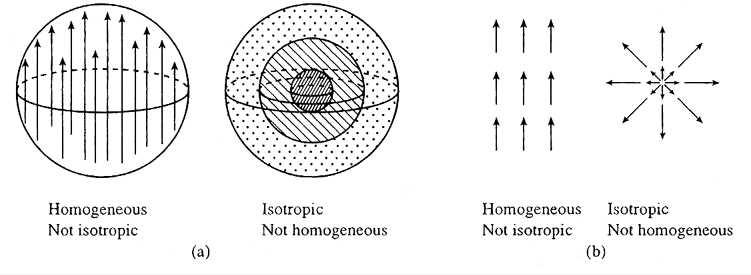
\includegraphics[width=11cm, height=6cm]{hom.jpg}
\end{center}
  \caption{\textit{Idea of homogeneous and isotropic universe in 3-d}}
\end{figure}
\pagebreak
There are two methods to derive the cosmological equations- (1)-using Newtonian mechanics and (2)-using Einstein's equations of General Relativity. We will derive it by both methods.\\ \\
\textit{1. Using Newtonian mechanics:}\\ \\
We know that the universe is expanding. Therefore we need to separate the movement based on the particle relative to the background, and the movement due to the expansion. The Cosmological Principle postulates that at each location in the universe one can define a hypothetical observer to whom the universe appears isotropic and homogeneous. Such observers are called \textit{comoving observers}, and we can define a \textit{comoving coordinate system}, in which these observers remain at rest; this means that comoving coordinates are expanding along with the universe. The proper distance $\mathbf{r}$ is the distance between two regions of space at a constant cosmological time. As the universe expands, the proper distance between two comoving observers increases over time.  By definition, the comoving distance between two comoving regions of space remains fixed at all times. It is related to the proper distance as follows : \\
\begin{equation}
\mathbf{r}(t)=a(t) \mathbf{x}
\end{equation}
where $\mathbf{r}$ is called the proper coordinate, $\mathbf{x}$ is called the comoving coordinate and $a(t)$ is the scale factor. Therefore relative velocity between two points is\\
\begin{equation*}
\begin{aligned} 
\mathbf{v}_{21} &=\frac{d}{d t}\left(\mathbf{r}_{2}-\mathbf{r}_{1}\right) \\ &=\dot{a}\left(\mathbf{x}_{2}-\mathbf{x}_{1}\right) \\ &=\frac{\dot{a}}{a}\left(\mathbf{r}_{2}-\mathbf{r}_{1}\right) 
\end{aligned}
\end{equation*} 
By generalizing this formula between any two points, and defining the \textit{Hubble’s parameter} $H(t)=\frac{\dot{a}}{a}$ ,we get the Hubble's law:\\
\begin{equation}
\mathbf{v}=H(t) \mathbf{D}
\end{equation} \\ 
Now Imagine a sphere of uniform density $\rho(t)$, with a radius $R$. This sphere is assumed to expand according to the scale factor $a$, therefore we can define a comoving radius $X_{R}$, and the radius of the sphere as a function of time is \\
\begin{equation}
R(t)=X_{R} a(t)
\end{equation}
The sphere is assumed to follow Newtonian dynamics and each point of sphere is been attracted gravitationally to all the other points. Since the whole system has only the degree of freedom of the scale factor, the
equation of motion of a single point can be used to determine the evolution of the whole system. Let’s take a small mass mp, placed at a comoving distance $x_{p}$ from the center. The potential energy $E_{p}$ is\\
\begin{equation*}
E_{p}=-\frac{G M_{p} m_{p}}{r_{p}}
\end{equation*}
where $M_{p}$ is the mass contained in a sphere of radius $r_{p}$ :\\
\begin{equation*}
M_{p}=\frac{4}{3} \pi \rho r_{p}^{3}
\end{equation*}
The resulting potential energy is: \\
\begin{equation*}
E_{P}=-\frac{4}{3} \pi \rho G m_{p} r_{p}^{2}
\end{equation*}
The kinetic energy is \\
\begin{equation*}
E_{K}=\frac{1}{2} m_{p} \dot{r}_{p}^{2}=\frac{1}{2} m_{p} \frac{\dot{a}^{2}}{a^{2}} r_{p}^{2}
\end{equation*} 
From the law of conservation of energy,\\
\begin{equation*}
E_{t o t}=E_{P}+E_{K}
\end{equation*}
therefore,\\
\begin{equation*}
E_{t o t}=-\frac{4}{3} \pi \rho G m_{p} r_{p}^{2}+\frac{1}{2} m_{p} \dot{r}_{p}^{2}
\end{equation*}
Isolating the derivative of a\\
\begin{equation}
\left(\frac{\dot{a}}{a}\right)^{2}=\frac{8 \pi G}{3} \rho+\frac{2}{m_{p} r_{p}^{2}} E_{t o t}
\end{equation}
Differentiating the potential energy gives the force on the mass \\
\begin{equation}
F_{p}=-\frac{d E_{P}}{d r}=\frac{8}{3} \pi \rho G m_{p} r_{p}
\end{equation}
Einstein thought that the universe
was static, end therefore introduced a second force which could counteract the non
zero acceleration, for all $r_{p}$ ,and a non-empty universe. Since this force had to be of the right intensity at all r, its form is bound to have the same dependence on the radius as the gravitational force, leading to a potential energy of this form: \\
\begin{equation}
E_{\Lambda}=\text { const } \times r_{p}^{2}=-m \frac{\Lambda c^{2}}{6} r_{p}^{2}
\end{equation}
where the dependence on $m$ is obliged by the condition that all forces and accelerations in the previous formulas are proportional to it, while the various constants are due to the relativistic derivation of the same concept. The total energy is rewritten as \\
\begin{equation}
E_{t o t}=-\frac{m_{p} r_{p}^{2}}{2} \frac{K c^{2}}{6 a^{2}}
\end{equation}
Hence with the added term for cosmological constant and new definitions, we can write the \textit{First Friedmann Equation as}:\\
\begin{equation}
\left(\frac{\dot{a}}{a}\right)^{2}=\frac{8 \pi G}{3} \rho-\frac{K c^{2}}{a^{2}}+\frac{\Lambda c^{2}}{3}
\end{equation}
This equation need to be solved for two functions: $a(t)$ and $\rho(t)$. The Newtonian model provides an equation for $\rho(t)$: since the mass in the sphere is always the same, as the sphere expands the density decrease, with a relation that is the inverse of the increment in volume. Therefore 
$\rho \propto \frac{1}{a^{3}}$ and differentiating  with respect to time gives:\\
\begin{equation}
\dot{\rho} \propto-3 \frac{\dot{a}}{a^{2}}
\end{equation}
dividing the equation for $\dot{\rho}$ and $\rho$ gives:\\
\begin{equation}
\dot{\rho}=-3 H \rho
\end{equation}
Now, multiplying (24) by $a^2$ and differentiating w.r.t time, \\
\begin{equation*}
2\dot{a}\ddot{a}=\frac{8 \pi G}{3}\left(\dot{\rho}a^{2}+ 2\dot{a}a \rho\right)+\frac{\Lambda c^{2}}{3} 2\dot{a}a
\end{equation*}
dividing by $2\dot{a}a$, we get the \textit{Second Friedmann Equation} \\
\begin{equation}
\frac{\ddot{a}}{a}=-\frac{8 \pi G}{6} \rho+\frac{\Lambda c^{2}}{3}
\end{equation}
Hence the final 2 Friedmann equations are:\\
\begin{equation}
\left(\frac{\dot{a}}{a}\right)^{2}=\frac{8 \pi G}{3} \rho-\frac{K c^{2}}{a^{2}}+\frac{\Lambda c^{2}}{3}
\end{equation}
\begin{equation}
\frac{\ddot{a}}{a}=-\frac{8 \pi G}{6} \rho+\frac{\Lambda c^{2}}{3}
\end{equation} \\ 

\textit{2. Using Einstein's equations:} \\ \\
The key notion of General relativity is that \textit{the presence of mass/energy determines the geometry of space and the geometry of space determines the motion of mass/energy.} Einstein’s general theory of relativity is a geometric theory of gravity— gravitational phenomena are attributed as reflecting the underlying curved spacetime. An invariant (with respect to coordinate transformations) interval is related to coordinates of the spacetime manifold through the metric in the form of:\\
\begin{equation}
d s^{2}=g_{\mu \nu} d x^{\mu} d x^{\nu}
\end{equation}
The Greek indices range over (0, 1, 2, 3) with $x^{0} = ct$ and the metric  $g_{\mu \nu}$ is a 4 $\times$ 4 matrix.\\
 We study the universe that follows from the cosmological principle. The cosmological principle states that: \textit{at each epoch (i.e. each fixed value of cosmological time $t$) the universe is homogeneous and isotropic. It presents the same aspects (except for local irregularities) from each point.} Due  to  the  symmetries that this principle implies, we can set a cosmological time  which allows us to have a reference time to study the universe dynamics.\\
Now, the field equation in Newton’s theory of gravity, when written in terms of the gravitational potential $\phi(x)$, is given by:\\
\begin{equation}
\nabla^{2} \phi=4 \pi G \rho
\end{equation}
where $\rho$ is the density of mass and $G$ is the Newton's constant. The
Newtonian theory is not a dynamic field theory as it does not provide a description of time evolution. Namely, it is the static limit of some field theory, thus has no field propagation. The Newtonian equation of motion is \\
\begin{equation}
\frac{d^{2} \mathbf{r}}{d t^{2}}=-\nabla \Phi
\end{equation}
Einstein in his theory of gravity, obtained the relativistic generalisations of equations (25) and (26). Since in relativity space and time are treated on equal footing, a successful relativistic program will automatically yield a dynamical theory as well. Einstein's field equations can be written as $[6]$
\begin{equation}
G_{\mu \nu}+\Lambda g_{\mu \nu}=k T_{\mu \nu}
\end{equation}
where $\Lambda$ and $k$ are undetermined constants.The constant $k$ is determined by demanding that Newton's gravitational field equation comes out right but $\Lambda$ remains arbitrary.The value of $k$ comes out to be  $\frac{8 \pi G}{c^{4}}$\\
The Einstein's tensor $G_{\mu \nu}$ is defined as:\\
\begin{equation}
G_{\mu \nu}=R_{\mu \nu}-\frac{1}{2} R g_{\mu \nu}
\end{equation}
Hence EFE can be written(in tensor form) as: \\
\begin{equation}
R_{\mu \nu}-\frac{1}{2} R g_{\mu \nu}+\Lambda g_{\mu \nu}=\frac{8 \pi G}{c^{4}} T_{\mu \nu}
\end{equation}
where $R_{\mu \nu}$ is the Ricci curvature tensor, R is the scalar curvature, $g_{\mu \nu}$ is the metric tensor, $\Lambda$ is the  cosmological constant, $G$ is the Newton's gravitation constant, $T_{\mu \nu}$ is the stress-energy tensor, and $c$ is the speed of light in vacuum.The Einstein's field equations are a set of symmetric 4$\times$ 4 tensors each having 10 components. The equations are nonlinear, but they have a wellposed initial-value structure – that is, they determine future values of $g_{\mu \nu}$ from given initial data. However, one point must be made: since $g_{\mu \nu}$ are the components of a tensor in some coordinate system, a change in coordinates induces a change in them. In particular, there are four coordinates, so there are four arbitrary functional degrees of freedom among the ten $g_{\mu \nu}$. It should be impossible, therefore, to determine all ten $g_{\mu \nu}$ from any initial data, since the coordinates to the future of the initial moment can be changed arbitrarily. In fact, Einstein’s equations have exactly this property: the Bianchi identities\\
\begin{equation}
G_{ ; \nu}^{\mu \nu}=0
\end{equation}
 in  Einstein  tensor $G_{\mu \nu}$  there  is  a  Ricci-tensor  and  a  Ricci  escalar.   The  metric  with  which  weare going to calculate them is the one that we need to particularise  our  final  expressions  for  the  homogeneous and  isotropic  universe.   Therefore  now  we  have  to  find a metric $g_{\mu \nu}$ that includes all the different aspects of the cosmological principle. The metric is Robertson-Walker metric:\\
\begin{equation}
\mathrm{d} s^{2}=c^{2} \mathrm{d} t^{2}-a^{2}(t)\left[\frac{\mathrm{d} r^{2}}{1-k r^{2}}+r^{2}\left(\mathrm{d} \theta^{2}+\sin ^{2} \theta \mathrm{d} \phi^{2}\right)\right]
\end{equation}
The Robertson-Walker metric describes an isotropic universe, because it does not have crossed terms between time and space so there is not any priviledged direction$[6]$. And it also describes the homogeneous universe because of the spherical symmetry. The factor $a(t)$ is called the scale factor and it is the temporal dependence between the relative distance of two points of the universe. The scale factor is defined to be 1 in the present time. The parameter $k$ specifies the curvature of space. For the flat space space it's value is $0$. It can take three values-$+1$, $-1$ or $0$. From now on the time dependence of the scale factor can be implicit, so $a(t)\equiv a$. \\
We need the Ricci tensor and Ricci scalar to particularise Einstein's equations for a homogeneous and isotropic universe. First we calculate the components of metric tensor and then substitute them in Christoffel symbol formula which is\\
\begin{equation}
\Gamma_{j i}^{l}=\frac{1}{2} g^{l m}\left(\frac{\partial g_{m i}}{\partial x^{j}}+\frac{\partial g_{m j}}{\partial x^{i}}-\frac{\partial g_{i j}}{\partial x^{m}}\right)
\end{equation}
We will then use it to get Riemann tensor which is connected to Christoffel symbol as:\\
\begin{equation}
R_{k j i}^{l} = \frac{\partial \Gamma_{k j}^{l}}{\partial x^{i}}-\frac{\partial \Gamma_{k i}^{l}}{\partial x^{j}}+\Gamma_{k j}^{m} \Gamma_{m i}^{l}-\Gamma_{k i}^{m} \Gamma_{m j}^{l}
\end{equation}\\
\textit{Calculating metric tensor:}\\
The metric tensor $g_{i j}$ is a function which tells us how to compute the distance between any two points in a given space.  Its components can be viewed as multiplication factors which must be placed in front of the differential displacements $dx_{i}$ in a generalized Pythagorean theorem:\\
\begin{equation}
d s^{2}=g_{11} d x_{1}^{2}+g_{12} d x_{1} d x_{2}+g_{22} d x_{2}^{2}+\ldots .
\end{equation}
In Euclidean space,$g_{i j}=\delta_{i j}$. Now for Robertson-Walker metric, we set :\\
\begin{align*}
x^{0}&=ct &  x^{1}&=r &  x^{2}&=\theta &  x^{3}&=\phi
\end{align*}
The non-zero components of metric tensor $g_{i k}$ and $g^{i k}$ using equation (24) can be calculated as :\\
\begin{equation}
g_{00}=1, \quad g_{11}=-\frac{a^{2}}{1-k r^{2}}, \quad g_{22}=-a^{2} r^{2}, \quad g_{33}=-a^{2} r^{2} \sin ^{2} \theta
\end{equation}
\begin{equation}
g^{00}=1, \quad g^{11}=-\frac{1-k r^{2}}{a^{2}}, \quad g^{22}=-\frac{1}{a^{2} r^{2}},  g^{33}=-\frac{1}{a^{2} r^{2} \sin ^{2} \theta}
\end{equation}
Next we calculate the Christoffel symbols of Robertson-Walker metric:\\ \\
\textit{Calculating Christoffel Symbols:}\\ \\
Robertson-Walker  metric  is  diagonal  and has  a  symmetric  connection,  so  the  majority  of  the Christoffel symbols will be symmetric or null. The non zero components of $\Gamma_{j i}^{l}$ are :\\
\begin{align*}
\Gamma_{01}^{1}&=\Gamma_{02}^{2}=\Gamma_{03}^{3}=\frac{1}{c} \frac{\dot{a}}{a}
\end{align*}
\begin{align*}
\Gamma_{11}^{0}&=\frac{a \dot{a}}{c\left(1-k r^{2}\right)} &  \quad \Gamma_{22}^{0}&=\frac{a \dot{a} r^{2}}{c} &  \quad \Gamma_{33}^{0}&=\frac{a \dot{a} r^{2} \sin ^{2} \theta}{c}
\end{align*}
\begin{align*}
\Gamma_{11}^{1}&=\frac{k r}{1-k r^{2}} &  \quad \Gamma_{12}^{2}&=\Gamma_{13}^{3}=\frac{1}{r}
\end{align*}
\begin{align*}
\Gamma_{22}^{1}&=-r\left(1-k r^{2}\right) &  \quad \Gamma_{33}^{1}&=-r\left(1-k r^{2}\right) \sin ^{2} \theta
\end{align*}
\begin{align*}
\Gamma_{33}^{2}&=-\sin \theta \cos \theta &  \quad \Gamma_{23}^{3}&=\cot \theta
\end{align*}\\ 
\textit{Calculating Riemann tensor:}\\ \\
Riemann tensor is defined as:\\
\begin{equation}
R_{k j i}^{l} = \frac{\partial \Gamma_{k j}^{l}}{\partial x^{i}}-\frac{\partial \Gamma_{k i}^{l}}{\partial x^{j}}+\Gamma_{k j}^{m} \Gamma_{m i}^{l}-\Gamma_{k i}^{m} \Gamma_{m j}^{l}
\end{equation}
Ricci Tensor $R_{k i}$ is the contraction of the Riemann tensor:\\
\begin{equation}
R_{k i} \equiv R_{k j i}^{l}
\end{equation}
and Ricci scalar $R$ is the contraction of Ricci tensor:\\
\begin{equation}
R=g^{i k} R_{i k}
\end{equation} 
Therefore we will calculate only those components of Riemann tensor which have the same top index as the middle bottom one. These components are enough to calculate Ricci tensor.\\
\begin{equation}
R_{0 0}=R_{t m t}^{m}=R_{t r l}^{r}+R_{t \theta t}^{\theta}+R_{t \phi t}^{\phi}= \frac{3}{c^{2}} \frac{\ddot{a}}{a}
\end{equation}
\begin{equation}
R_{1 1}=R_{2 2}=R_{3 3}=\frac{1}{c^{2}}\left(\frac{\ddot{a}}{a}+\frac{2 \dot{a}^{2}+2 k c^{2}}{a^{2}}\right)
\end{equation}
Finally, we can write Ricci Scalar as:\\
\begin{equation}
R=g^{i k} R_{i k} = \frac{6}{c^{2}}\left(\frac{\ddot{a}}{a}+\frac{\dot{a}^{2}+k c^{2}}{a^{2}}\right)
\end{equation} \\
\textit{Energy-momentum tensor $T_{\mu \nu}$}:\\ \\
We can think about the universe being filled by a perfect fluid as this kind of fluid follows the cosmological principle. By definition a perfect fluid is the one that is isotropic,which  means  that  it  has  to  look  equal  to  us  in  every direction we can move.  Then, the macroscopic speed of the fluid cannot have a privileged direction, so it has only temporal component i.e $u^{\alpha}=(1,0,0,0)$. The explicit expression for the energy momentum tensor is:\\
\begin{equation}
T_{\mu \nu}=(\rho+p) u_{\mu} u_{\nu}-p g_{\mu \nu}
\end{equation}
where $u_{\alpha}$ is the macroscopic speed of the medium. Now we can find the energy-momentum tensor for a perfect fluid. It has only diagonal components:\\
\begin{align*}
T_{t t}&=\rho g_{t t} &  T_{i i}&=-p g_{i i}
\end{align*}
Now we have calculated all the components of Einstein's equation. So now we have to plug all the elements to Einstein's Equations(29). The only equations that will be different from the null one  are  those  which  have the same indexes, since our metric is diagonal$[6]$. Therefore we start with the temporal part.\\
\begin{equation}
R_{t t}-\frac{1}{2} R g_{t t}-\Lambda g_{t t}=8 \pi G \rho u_{t} u_{t}
\end{equation}
\begin{equation}
-3 \frac{\ddot{a}}{a}+3 \frac{\ddot{a}}{a}+3\left(\frac{\dot{a}}{a}\right)^{2}+3 \frac{1}{K^{2} a^{2}}-\Lambda=8 \pi G \rho(t)
\end{equation}
Rearranging the terms,\\
\begin{equation}
\left(\frac{\dot{a}(t)}{a(t)}\right)^{2}=\frac{8 \pi G}{3} \rho(t)+\frac{\Lambda}{3}-\frac{1}{K^{2} a^{2}(t)}
\end{equation}
This is the \textit{first Friedmann equation}. We now take the spatial part:\\
\begin{equation}
R_{i i}-\frac{1}{2} R g_{i i}-\Lambda g_{i i}=8 \pi G(-p) g_{i i}
\end{equation}
therefore,\\
\begin{equation}
-\frac{\ddot{a}}{a}-2\left(\frac{\dot{a}}{a}\right)^{2}-\frac{2}{K^{2} a^{2}}+3 \frac{\ddot{a}}{a}+3\left(\frac{\dot{a}}{a}\right)^{2}+\frac{3}{K^{2} a^{2}}-\Lambda=-8 \pi G p
\end{equation}
or,\\
\begin{equation}
\frac{\ddot{a}(t)}{a(t)}+\frac{1}{2}\left(\frac{\dot{a}(t)}{a(t)}\right)^{2}=-4 \pi G p+\frac{\Lambda}{2}-\frac{1}{2} \frac{1}{K^{2} a^{2}(t)}
\end{equation}
Now we do 2$\times$(49)- (46), we get:\\
\begin{equation}
\frac{\ddot{a}(t)}{a(t)}=-\frac{4 \pi G}{3}(\rho(t)+3 p)+\frac{\Lambda}{3}
\end{equation}
This is the \textit{second Friedmann equation}.\\
Hence in both relativistic and Newtonian Friedman equations derivation, we have arrived to dynamical expressions  that  describe a non-static  isotropic and homogeneous universe in general conditions. 

\pagebreak

\section*{{$\mathbf{III}$. Constructing Lagrangian and Hamiltonian structure using time independent constant of motion}}

In this section we are going to explain in detail how can we write the Lagrangian and Hamiltonian structure for a system  starting from just one time independent constant of motion$[1]$.\\
Consider a system of 2$n$ first order differential equationsfor 2n variables $x^{a}$,\\
\begin{equation}
\dot{x}^{a}=f^{a}\left(x^{b}\right), \quad a, b=1,2,3, \ldots, 2 n
\end{equation}
The Hamiltonian structure for the system consists of Hamiltonian(H), a Poisson Bracket relation which can be described in terms of a matrix called Poisson Bracket matrix $J^{a b}$. Poisson Bracket can be written in the following form for defining $J$, $[5]$\\
\begin{equation}
\{F,G\}=\frac{\partial F} {\partial z^{i}} J^{i j}\frac{ \partial G}{\partial z^{j}} 
\end{equation}
where,\\
\begin{equation}
J=\left( \begin{array}{rr}{0} & {I} \\ {-I} & {0}\end{array}\right)
\end{equation}
where $I$ is the 3$N$ dimensional unit matrix. The significance of (25) is that the Poisson Bracket relation is covariant under arbitrary transformations of the phase coordinates $z^{i}$ $[4]$, that is if\\
\begin{equation}
\overline{z}^{i}=\overline{z}^{i}(z)
\end{equation}
are new coordinates, $\overline{F}(\overline{z})$ is the function $F(z)$ expressed in the new coordinates,and\\
\begin{equation}
\overline{J}^{i j}=\frac{\partial \overline{z}^{i}}{\partial z^{m}}{J}^{m n}\frac{\partial \overline{z}^{j}}{\partial z^{n}}
\end{equation}
transforms as rank-two contravariant tensor.And since Poisson bracket follows the antisymmetric property and Jacobi identity$[4]$,\\
\begin{equation}
J^{i j}=-J^{j i}
\end{equation}
and\\
\begin{equation}
J^{i m}\frac{\partial J^{j k}}{ \partial z^{m}} + J^{j m}\frac{\partial J^{k i}}{ \partial z^{m}} + J^{k m}\frac{\partial J^{i j}}{ \partial z^{m}} = 0
\end{equation}
changing the indices from $i$, $m$, $j$, $k$ to $c$, $d$, $a$, $b$ and writing the above expression in compressed form,\\
\begin{equation}
J_{, d}^{a b} J^{d c}+J_{, d}^{b c} J^{d a}+J_{, d}^{c a} J^{d b} \equiv 0
\end{equation}
this is the well known Jacobi identity for Poisson bracket matrix. Hence hamilton equations can be written as:\\
\begin{equation}
f^{a}\left(x^{c}\right)=J^{a b} \frac{\partial H}{\partial x^{b}} \equiv\left[x^{a}, H\right]
\end{equation}
If the Lagrangian of the system is known, then we can obtain the Hamiltonian structure(canocical momenta, a Hamiltonian and Poisson Bracket relations) using standard procedures of textbooks. But if the Lagrangian is not known or if it does not exist we cannot apply the standard procedure.In this section we present new approach in writing the Hamiltonian structure of a second order system where one constant of motion allows for the construction of the Hamiltonian and Lagrangian structures as well as the complete integration of the problem. This new approach is applied to find the Lagrangian and Hamiltonian of cosmological equations derived in the previous chapter.\\

\subsection*{\textit{$\mathbf{III.I}$. Construction of Hamiltonian Structure}}
Let us consider a system of two first order diffrential equations for two variables $x^{a}$ \\
\begin{equation}
\dot{x}^{a}=f^{a}\left(x^{b}\right) . \quad a, b=1,2
\end{equation}
We assume that one time independent constant of motion $C_{1}(x^{b})$ is known. Then this constant satisfies the following equation:\\
\begin{equation}
\frac{\partial C_{1}}{\partial x^{a}}\dot{x}^{a}=0
\end{equation}
i.e \\
\begin{equation}
\frac{\partial C_{1}}{\partial x^{a}} f^{a}\left(x^{b}\right) \equiv 0 . \quad a, b=1,2
\end{equation}
For constructing the Hamiltonian structure for the system requires the knowledge of Hamiltonian(H) and Poisson bracket matrix $J^{a b}$.In two dimensions there is essentially one antisymmetric matrix, hence\\
\begin{equation}
J^{a b}=\left( \begin{array}{cc}{0} & {\mu\left(x^{b}\right)} \\ {-\mu\left(x^{b}\right)} & {0}\end{array}\right)
\end{equation}
The function $\mu(x^{b})$ is determined by Hamilton's equations condition\\
\begin{equation*}
f^{a}\left(x^{c}\right)=J^{a b} \frac{\partial H}{\partial x^{b}}
\end{equation*}
If we choose $H=C_{1}$\\,
\begin{equation}
f^{a}\left(x^{c}\right)=J^{a b} \frac{\partial C_{1}}{\partial x^{b}}
\end{equation}
Now due to (35) the gradient of $C_{1}$ is perpendicular to $f$, therefore 
$J^{a b} \frac{\partial C_{1}}{\partial x^{b}}$ is parallel to $f^{a}$ in 2-dimensional space. Thus (37) determines the function $\mu(x^{b})$ uniquely. Hence if a time independent constant of motion $C_{1}(x^{b})$ is known, the Hamiltonian structure is defined by choosing the time independent constant as the Hamiltonian and the Poisson Bracket matrix is completely determined by Hamilton's equation conditions.\\

\subsection*{\textit{$\mathbf{III.II}$. Construction of Lagrangian Structure}}
Suppose $(q_{1}, q_{2},....q_{n},(p_{1}, p_{2},....p_{n})$ are the canonical coordinates on a phase space. If each of them is expressed as a function of $u$ and $v$, then the Lagrange bracket of $u$ and $v$ is definied as,\\
\begin{equation}
[u, v]_{p, q}=\sum_{i=1}^{n}\left(\frac{\partial q_{i}}{\partial u} \frac{\partial p_{i}}{\partial v}-\frac{\partial p_{i}}{\partial u} \frac{\partial q_{i}}{\partial v}\right)
\end{equation}
If the structure is symplectic, then the canonical coordinates $(q,p)$ may be expressed as functions of coordinates $u$ and the matrix of Lagrange Brackets \\
\begin{equation}
\left[u_{i}, u_{j}\right]_{p, q}   , 1 \leq i, j \leq 2 n
\end{equation}
We will denote the Lagrange bracket matrix by $\sigma_{a b}$(changing the description from $p,q$ to $a,b$). The Lagrange Brackets matrix also follows antisymmetric condition and is the inverse of Poisson bracket matrix. Thus, \\
\begin{equation*}
\sigma_{a b}=\left( \begin{array}{cc}{0} & {\frac{1}{\mu\left(x^{b}\right)}} \\ {-\frac{1}{\mu\left(x^{b}\right)}} & {0}\end{array}\right)
\end{equation*}
\begin{equation*}
\sigma_{a b}=-\sigma_{b a}
\end{equation*}
and,
\begin{equation}
J^{a b} \sigma_{b c}=-\delta^{a}_{c}
\end{equation} 
Now the Hamilton's equations can be written as \\
\begin{equation}
\dot{x}^{a}=J^{a b} \frac{\partial C_{1}}{\partial x^{b}}
\end{equation}
Left Multiplying both sides by $\sigma_{c a}$ we get the Lagrangian form of Hamilton's equations:\\
\begin{equation}
\sigma_{c a} \dot{x}^{a}+\frac{\partial C_{1}}{\partial x^{c}}=0
\end{equation} 
The Lagrangian $L(q,\dot{q})$ can be written as:\\
\begin{equation}
L= p\dot{q} - H
\end{equation}
Now consider the Lagrangian $L=L\left(x^{a}, \dot{x}^{b}\right)$\\
\begin{equation}
L=L\left(x^{a}, \dot{x}^{b}\right)=l_{1}\left(x^{a}\right) \dot{x}^{1}-H
\end{equation}
Since we made the choice $H=C_{1}(x^{b})$, therefore \\
\begin{equation}
L=L\left(x^{a}, \dot{x}^{b}\right)=l_{1}\left(x^{a}\right) \dot{x}^{1}-C_{1}\left(x^{a}\right)
\end{equation}
where $l_{1}(x^{a})$ is defined by \\
\begin{equation}
\frac{\partial l_{1}}{\partial x^{2}}=\frac{1}{\mu}
\end{equation}
Since $a$ and $b$ both take two values 1,2 we can write the Euler-Lagrange equations for (46):\\
\begin{equation}
\frac{\partial l_{1}}{\partial x^{2}} \dot{x}^{2}+\frac{\partial C_{1}}{\partial x^{1}}=0
\end{equation}
and \\
\begin{equation}
-\frac{\partial l_{1}}{\partial x^{2}} \dot{x}^{1}+\frac{\partial C_{1}}{\partial x^{2}}=0
\end{equation}
These are equivalent to the Hamilton's equations (43). the function $l_{1}(x^{a})$ is determined upto and addition of arbitrary function $f_{1}(x^{1})$. This addition modifies the Lagrangian (45) by a total time derivative, hence Euler-Lagrange equations (47) and (48) remain invariant under the change.\\

\textit{Example:Dynamics of a general second order system} \\ \\
Consider a second order system defined as:\\
\begin{equation}
\ddot{q}=F(q) G(\dot{q})
\end{equation}
This second order equation can be written as two dimensional first order system.So we define:\\
\begin{equation}
x^{1} \equiv q
\end{equation}
and,\\
\begin{equation}
x^{2} \equiv \dot{q}
\end{equation}
The equations of motion can be written as:\\
\begin{equation}
\dot{x}^{1}=x^{2}
\end{equation}
and,
\begin{equation}
\dot{x}^{2}=F\left(x^{1}\right) G\left(x^{2}\right)
\end{equation}
Now we have to find the time independent constant of motion $C_{1}$. Therefore we have to write equation (49) in the following form before integrating: \\
\begin{equation}
\frac{\ddot{q}}{G(\dot{q})}=F(q) 
\end{equation}
Integrating, we get\\
\begin{equation}
\int\frac{\ddot{q}}{G(\dot{q})}dq = \int F(q) d q + C_{1}
\end{equation}
or,\\
\begin{equation}
\int\frac{\ddot{q}}{G(\dot{q})}\dot{q}dt = \int F(q) d q + C_{1}
\end{equation}
or,\\
\begin{equation}
\int\frac{\dot{q}}{G(\dot{q})}d\dot{q} = \int F(q) d q + C_{1}
\end{equation}
Hence time independent constant $C_{1}$ can be written as:\\
\begin{equation}
C_{1}(q, \dot{q})=-\int F(q) d q+\int \frac{\dot{q}}{G(\dot{q})} d \dot{q}
\end{equation}
Therefore, the hamiltonian $H$ is given as:\\
\begin{equation}
H\left(x^{1}, x^{2}\right)=-\int F\left(x^{1}\right) d x^{1}+\int \frac{x^{2}}{G\left(x^{2}\right)} d x^{2}
\end{equation}
and the Poisson Bracket matrix can be written as \\
\begin{equation}
J^{a b}=\left( \begin{array}{cc}{0} & {G\left(x^{2}\right)} \\ {-G\left(x^{2}\right)} & {0}\end{array}\right)
\end{equation}
The momentum $p$ can be written as:\\
\begin{equation}
\dot{p}=-\frac{\partial H}{\partial \dot{q}}
\end{equation}
hence momentum $p$ is given as\\
\begin{equation}
p=\int \frac{d x^{2}}{G\left(x^{2}\right)}
\end{equation}
Consider the following functional form of $G(\dot{q})$:\\
\begin{equation}
G(\dot{q})=\dot{q}
\end{equation}
for this form the time independent constant, the Hamiltonian, and the canonical momentum takes the following form:\\
\begin{equation}
C_{1}=-\int F(q) d q+\dot{q}
\end{equation}
\begin{equation}
p=\int \frac{d \dot{q}}{\dot{q}}=\ln \dot{q}
\end{equation}
\begin{equation}
H(q, p)=-\int F(q) d q+e^{p}
\end{equation}
We will now apply the above approaches and results for obtaining the Lagrangian and Hamiltonian for the cosmological equations that we derived in chapter II.\\ \\
\textit{Lagrangian and Hamiltonian structure for the cosmological equations:}\\ \\
For writing the Lagrangian and Hamiltonian for cosmological equations we consider a special state of matter called dust for which $P=0$. And we will be focussing our discussion for the flat universe model i.e $k=0$ and  as of the present discussion we will not consider cosmological constant. Hence taking in account the points, Friedmann equations take the following form:
\begin{equation}
\left(\frac{\dot{a}}{a}\right)^{2}=\frac{8 \pi G}{3 c^{2}} \rho
\end{equation}
\begin{equation}
2\frac{\ddot{a}}{a} + \left(\frac{\dot{a}}{a}\right)^{2} = 0
\end{equation}
Now, substituting the value of $\left(\frac{\dot{a}}{a}\right)^{2}$ from (94) into (95) we get:\\
\begin{equation}
2\frac{\ddot{a}}{a} + \frac{8 \pi G}{3 c^{2}} \rho=0
\end{equation}
or,\\
\begin{equation}
\ddot{a}= -\left(\frac{4 \pi G}{3 c^{2}} \rho\right) a
\end{equation}
From equation (20),\\
\begin{equation}
\frac{\dot{\rho}}{\rho} =-3 \frac{\dot{a}}{a^{2}}
\end{equation}
Integrating both sides, we get\\
\begin{equation}
\rho = \frac{k_{1}}{a^{3}}
\end{equation}
Substituting $\rho$ in (97)
\begin{equation}
\ddot{a}= -\left(\frac{4 \pi G}{3 c^{2} a^{2}} \right) k_{1}
\end{equation}
Now we find the time independent constant for (100). Choosing $x^{1}=a$ and $x^{2}=\dot{a}$ we can write the constant $C_{1}$ using (85) as:\\
\begin{equation}
C_{1}= -\left(\frac{4 \pi G}{3 c^{2} a} \right) k_{1} +\frac{\dot{a}^{2}}{2}
\end{equation}
Putting $k_{1}=\rho a^{3}$
\begin{equation}
C_{1}=-\left(\frac{4 \pi G}{3 c^{2} }\right) \rho a^{2} +\frac{\dot{a}^{2}}{2}
\end{equation}
Dividing throughout by $a^{2}$ and substituing the value of $\left(\frac{\dot{a}}{a}\right)^{2}$ from first Friedmann equation, we get:\\
\begin{equation}
C_{1}=0
\end{equation}
Hence we can write another constant $C_{1}'$ as:\\
\begin{equation}
C_{1}'= f(a,\dot{a}) C_{1}
\end{equation}
Now differentiating $C_{1}'$ w.r.t time
\begin{equation}
\frac{dC_{1}'}{dt}= f'(a,\dot{a})\dot{a}C_{1} + f(a,\dot{a})\dot{C_{1}}=0
\end{equation}
Hence we have seen that:\\
I. $C_{1}$  is a constant of motion and hence can be taken as the Hamiltonian(from previous discussion in this chapter). \\
II. The first Friedmann equation can be satisfied provided $C_{1}$ vanishes.\\
III. We can multiply $C_{1}$ by any function of $a$ and $\dot{a}$ to get a new constant $C_{1}'$(which can also be taken as the Hamiltonian) which satisfies both the cosmological equations. \\
Now the task that is remained is to choose $f$. We will choose the function $f(a,\dot{a})$ in such a way that the Hamiltonian whose role is played by $C_{1}$ is the linear combination of :\\
1. Matter Hamiltonian$(\mathcal{H}_{m})$ - which depends on density $\rho$ or $k_{1}$, and \\
2. Gravitational Hamiltonian$(\mathcal{H}_{g})$ - which depends on $a$ and $\dot{a}$.\\
i.e \\
\begin{equation}
\mathcal{H}=\mathcal{H}_{g}+\mathcal{H}_{m}
\end{equation}
Therefore we choose $f$ as :\\
\begin{equation}
f(a,\dot{a})=-\frac{3 c^{2}}{4 \pi G} a
\end{equation}
hence the Hamiltonian $\mathcal{H}$ can be written as:
\begin{equation}
\mathcal{H} = C_{1}' =f(a, \dot{a}) C_{1}= k_{1} - \frac{3 c^{2}}{8 \pi G} a \dot{a}^{2}
\end{equation}
Hence $\mathcal{H}=\mathcal{H}_{g}+\mathcal{H}_{m}$ , where
\begin{equation}
\mathcal{H}_{m} = k_{1}=\rho a^{3}  ,   \mathcal{H}_{g} = -\frac{3 c^{2}}{8 \pi G} a \dot{a}^{2}
\end{equation}\\
Now the Hamilton's equations are given as:
\begin{equation}
\frac{\partial \mathcal{H}}{\partial x^{2}} = \mu \dot{x^{1}}
\end{equation}
\begin{equation}
\frac{\partial \mathcal{H}}{\partial x^{1}}=-\mu \dot{x^{2}}
\end{equation}
where $\mu \dot{x^{1}}= \dot{q}$(in our case $\dot{a}$) and $\mu \dot{x^{2}}= -\dot{p}$. Hence \\
\begin{equation}
\mu = -\frac{3 c^{2}}{4 \pi G} a
\end{equation} 
therefore,\\
\begin{equation}
p=-\frac{3 c^{2}}{4 \pi G} a \dot{a}
\end{equation}
Now substituting $\dot{a}$ into $\mathcal{H}$, we get\\
\begin{equation}
\mathcal{H}=\mathcal{H}_{m} - \left(\frac{2 \pi G}{3 c^{2} a}\right) p^{2}
\end{equation}
This is our final expression for Hamiltonian. Now Lagrangian is given as :
\begin{equation}
\mathcal{L} = p\dot{q} - \mathcal{H}= p \frac{\partial \mathcal{H}}{\partial x^{2}} - \mathcal{H}
\end{equation}
Therefore,\\
\begin{equation}
\mathcal{L} = -\mathcal{H}_{m} + \frac{3 c^{2} a \dot{a}^{2}}{8 \pi G}
\end{equation}
This is our final expression for Lagrangian. We can verify through Hamilton's equations that the Hamiltonian given here gives back the cosmological equations we started with. Hence the functional form of our Hamiltonian is correct.
\pagebreak

\section*{{$\mathbf{IV}$. Constructing Lagrangian using the method of Jacobi-Jacobi's Last Multiplier(JLM)}}

In this chapter we will discuss about the link between an old method of Jacobi i.e Jacobi's last Multiplier(JLM) and the Lagrangian of a second order system$[2]$. It is well known fact that for any second order differential equation, there always exist a Lagrangian. But what is less known is that if we have the knowledge of a Jacobi Last Multiplier, we can always find the Lagrangian for that system. Also, the Multiplier provides a straightforward and easy method to derive the Lagrangian  whereas if one follows the standard procedure, one has to face lengthy and nonobvious mathematical steps to obtain a Lagrangian(and the corresponding Hamiltonian).\\
Many second order ordinary differential equations(ODEs) of the form $\ddot{x}=F(t,x,\dot{x})$ admit a Lagrangian description because of the existence of Jacobi Last Multiplier. Jacobi presented a series of lectures on dynamics in Berlin during 1847. Of the 38 lectures, three were devoted to what he termed an ‘un nouveau principe de la mécanique analytique’, which suggests that Jacobi thought that this was an important
development in the subject of Classical Mechanics. The Last Multiplier has never been particularly popular as a tool in the solution of problems in mechanics, but from time to time there have been applications.\\
Jacobi's Last Multiplier is a solution of the linear partial differential equation,$[3]$ \\
\begin{equation}
\frac{\mathrm{d} \log M}{\mathrm{d} t}+\sum_{i=1}^{n} \frac{\partial\left(a_{i}\right)}{\partial x_{i}}=0
\end{equation}
where $\partial_{t}+\sum_{i=1}^{n} a_{i} \partial_{x_{I}}$ is the vector field of the partial differential equation\\
\begin{equation}
A f=\frac{\partial f}{\partial t}+\sum_{i=1}^{n} a_{i}\left(x_{1}, \ldots, x_{n}\right) \frac{\partial f}{\partial x_{i}}=0
\end{equation}
or it's equivalent associated Lagrange system \\
\begin{equation}
\frac{\mathrm{d} x_{1}}{a_{1}}=\frac{\mathrm{d} x_{2}}{a_{2}}=\ldots=\frac{\mathrm{d} x_{n}}{a_{n}}=\frac{\mathrm{d} t}{1}
\end{equation}
An important property of the Last Multiplier is that the ratio of two multipliers, say $M/M'$, is a solution of (68)$[3]$, or equally a first integral of (69). Every Multiplier M is a solution of the linear partial differential equation\\
\begin{equation}
\frac{\partial\left(M a_{1}\right)}{\partial x_{1}}+\frac{\partial\left(M a_{2}\right)}{\partial x_{2}}+\cdots+\frac{\partial\left(M a_{n}\right)}{\partial x_{n}}=0
\end{equation} 
or it's equivalent, \\
\begin{equation}
\sum_{i=1}^{n} a_{i} \frac{\partial(\log M)}{\partial x_{i}}+\sum_{i=1}^{n} \frac{\partial a_{i}}{\partial x_{i}}=0
\end{equation}
conversly, every solution $M$ of this equation is a jacobi Last Multiplier.\\ \\
\textit{From JLM to Lagrangian:}\\ \\
We now present the link between the Lagrangian and Jacobi Last Multiplier for the second order ordinary differential equation$[2]$.\\ 
Consider a second order system\\
\begin{equation}
\ddot{y}=F(t, y, \dot{y})
\end{equation} 
From equation (67) we can write \\
\begin{equation}
\frac{d}{d t}(\log M)+\frac{\partial F}{\partial \dot{y}}=0
\end{equation}
or,\\
\begin{equation}
M=\exp \left[-\int \frac{\partial F}{\partial \dot{y}} d t\right]
\end{equation}
The relation between the Lagrangian and Jacobi Last Multiplier is:\\
\begin{equation}
\frac{\partial^{2} L}{\partial \dot{x}^{2}}=M
\end{equation}
which in our case can be written as \\
\begin{equation}
M=\frac{\partial^{2} L}{\partial \dot{y}^{2}}
\end{equation}
where $L=L(t,y,\dot{y})$ is the Lagrangian sought. This means that if know one Last Multiplier M, then we can obtain $L$ by two successive integrations:\\
\begin{equation}
L=\int\left(\int M d \dot{y}\right) d \dot{y}+f_{1}(t, y) \dot{y}+f_{2}(t, y)
\end{equation}
where $f_{1}$ and $f_{2}$ are arbitrary functions(constants of integration). Since every pair of Lagrangians which differ only by a total derivative with respect to time of a differentiable function gives rise to the same equations, we can define classes of equivalence among Lagrangians apart from the total derivative of an arbitrary function called a gauge function$[2]$. Hence we can choose a gauge function g(t,y) such that:\\
\begin{equation}
f_{1}=\frac{\partial g}{\partial y}
\end{equation}
\begin{equation}
f_{2}=\frac{\partial g}{\partial t}+f_{3}(t, y)
\end{equation}
Rewriting the Lagrangian in terms of gauge function, \\
\begin{equation}
L=\int\left(\int M d \dot{y}\right) d \dot{y}+\frac{d g}{d t}+f_{3}
\end{equation}
Now $g$ is an arbitrary gauge function but the equation (72) is derivable by above Lagrangian and therefore the Euler -Lagrange equation must give the second order differential equation we started with. This means $f_{3}$ is not arbitrary, but it has to satisfy the Euler-Lagrange equation:\\
\begin{equation}
-\frac{d}{d t}\left(\frac{\partial L}{\partial \dot{y}}\right)+\frac{\partial L}{\partial y}=0
\end{equation}
We now consider the following general form of equation of Painleve type and  find it's Lagrangian using above method:\\
\begin{equation}
\ddot{y}+A(y) \dot{y}^{2}+B(t, y) \dot{y}+C(t, y)=0
\end{equation}
Now, from equation (73) we can write,\\
\begin{equation}
\frac{d}{d t}(\log M)-2 A(y) \dot{y}-B(t, y)=0
\end{equation}
solving for multiplier $M$, we get \\
\begin{equation}
M=\exp \left[\int(2 A(y) \dot{y}+B(t, y)) d t\right]
\end{equation}   
Now we will consider different cases for different forms of $\ddot{y}$ :\\ \\
\textit{I.$\ddot{y}=0$} \\
In this case ,\\
\begin{equation}
\frac{d}{d t}(\log M)=0
\end{equation}
So we can take M=1 and therefore Lagrangian comes out to be \\
\begin{equation}
L=\frac{\dot{y}^{2}}{2}+\frac{d g}{d t}
\end{equation}\\ 

\textit{II.$\ddot{y}=\frac{\dot{y}^{2}}{y}$} \\
In this case,\\
\begin{equation}
\frac{d}{d t}(\log M)+\frac{2 \dot{y}}{y}=0
\end{equation}
therefore, \\
\begin{equation}
-\log M=\int 2 \frac{\dot{y}}{y} d t=\int 2 \frac{d y}{y}=2 \log y
\end{equation}
hence,\\
\begin{equation}
M=1 / y^{2}
\end{equation}
and \\
\begin{equation}
L=\frac{\dot{y}^{2}}{2 y^{2}}+\frac{d g}{d t}
\end{equation}\\ \\
\pagebreak

We will now apply the above procedure for finding the Multiplier and hence the Lagrangian for cosmological equations.\\
Comparing the second Friedman equation (95) with equation (132), we get,\\
\begin{equation}
A=\frac{1}{2 a} , B=0, C=0
\end{equation}
Now,form equation (134), we can calculate the multiplier M, which comes out be $a$, hence \\
\begin{equation}
M=a
\end{equation}
therefore using equation (130) to calulate the Lagrangian,\\
\begin{equation}
\mathcal{L}_{1} = \frac{a \dot{a}^{2}}{2} 
\end{equation}
which can also be written as :\\
\begin{equation}
\mathcal{L}_{1}=C_{1}\frac{a \dot{a}^{2}}{2}
\end{equation}
Since our Lagrangian has a gauge freedom we can add any constant to it say $\mathcal{L}_{2}$. Therefore we choose $\mathcal{L}_{2}$ as:\\
\begin{equation}
\mathcal{L}_{2} = \mathcal{H}_{m}
\end{equation}
therefore,\\
\begin{equation}
\mathcal{L}= C_{1} \frac{a \dot{a}^{2}}{2} + \mathcal{L}_{2}
\end{equation}
Now $\mathcal{H}$ can be found using legendre transformation:\\
\begin{equation}
\mathcal{H} = \mathcal{H}_{m} - C_{1} \frac{a \dot{a}^{2}}{2}
\end{equation}
As before the Hamiltonian $\mathcal{H}$ should vanish. Therefore,\\
\begin{equation}
\mathcal{H}_{m} = C_{1} \frac{a \dot{a}^{2}}{2}
\end{equation} 
Dividing both sides by $a^{3}$ and substituting for $\left(\frac{\dot{a}}{a}\right)^{2}$ from Friedmann equation, we get the value of the constant $C_{1}$\\
\begin{equation}
C_{1} = \frac{3 c^{2}}{4 \pi G}
\end{equation}
hence \\
\begin{equation}
\mathcal{L}= \frac{3 c^{2}}{8 \pi G} a \dot{a}^{2} - \mathcal{H}_{m}
\end{equation}
which is exactly the same Lagrangian we obtained in the previous chapter.

\pagebreak

\section*{\centerline{{$\mathbf{V}$. Conclusions}}}

From our analysis, we obtained the Lagrangian and Hamiltonian structure for cosmological equations by two completely different and independent methods and found that they are identical. In the first method we used the time independent constant of motion to find the Hamiltonian and then the Lagrangian. Whereas in second method we find the Lagrangian by a much more easy and efficient method of Jacobi's Last Multiplier.We found that the Lagrangian obtained has gauge freedom, which means we can add any constant to it without changing the functional form of Hamiltonian or any other quantity obtained from Lagrangian. Further we checked doing back calculation that the Lagrangian and Hamiltonian obtained give back the cosmological equation we started with.

\pagebreak

\section*{\centerline{{$\mathbf{V}$. References}}}

$[1]$- Sergio A. Hojman, "Construction of Lagrangian and Hamiltonian Structures starting from one Constant of Motion"arXiv:1403.0557v1 \\ \\
$[2]$- G. D Ambrosi,M.C Nucci "Lagrangians for equations of Painleve type by means of the Jacobi Last Multiplier" Journal of Nonlinear Mathematical Physics, Vol. 16, Suppl. (2009) 61–71 \\ \\
$[3]$- M C Nucci and P G L Leach1, "The Jacobi Last Multiplier and its
applications in mechanics", Phys. Scr. 78 (2008) 065011 (6pp)\\ \\ 
$[4]$- Rick Salmon, “Hamiltonian Fluid Mechanics”, Ann. Rev. Fluid Mech. 20, 225-256 (1988) \\ \\
$[5]$- Herbert Goldstein, “Classical Mechanics”, Addison– Wesley, Reading (1980) \\ \\
$[6]$- Jayant V.Narlikar, Fred Hoyle "Introduction to Cosmology", Second edition, Cambridge University Press(1993)







                                                                                                                                                                                                                                                                                                                                                                                                                                                                                                                                                                                                                                                                                                                                                                                                                                                                                                                                                                                                                                                                                                                                                                                                                                                                                                                                                                                                                                                                                                                                                                                                                                                                                                                                                                                                                                                                                                                                                                                                                                                                                                                                                                                                                                                                                                                                                                                                                                                                                                                                                                                                                                                                                                                                                                                                                                                                                                                                                                                                                                                                                                                                                                                                                                                                                                                                                                                                                                                                                                                                                                                                                                                                                                                                                                                                                                                                                                                                                                                                                                                                                                                                                                                                                                                                                                                                                                                                                                                                                                                                                                                                                                                                                                                                                                                                                                                                                                                                                                                                                                                                                                                                                                                                                                                                                                                                                                                                                                                                                                                                                                                                                                                                                                                                                                                                                                                                                                                                                                                                                                                                                                                                                                                                                                                  

\end{document}




